\documentclass[12pt,a4paper]{article}

\usepackage{geometry}
\geometry{
    left=2cm, 
    right=2cm,
    top=3cm,  
    bottom=2cm
}

\usepackage[english,spanish]{babel}
\usepackage[utf8]{inputenc}
\usepackage{amsmath}

\usepackage{graphicx}
\usepackage{wrapfig}

\usepackage{csquotes}
\usepackage{hyperref}
\usepackage[style=ieee]{biblatex}
\addbibresource{referencias.bib}

\usepackage{setspace}
\setstretch{1.5}
\setlength{\parindent}{0pt}

\usepackage{enumitem}

\begin{document}
\begin{titlepage}
    \begin{minipage}[c]{0.1\textwidth}
        
\includegraphics[width=\textwidth]{Resources/logo_unam.jpg}
    \end{minipage}
    \begin{minipage}{0.8\textwidth}
        \centering
        {\Large\textbf{Universidad Nacional Autónoma de México}\\}
        {\large\textbf{Escuela Nacional de Estudios Superiores\\\underline{Unidad Morelia}}}
    \end{minipage}
    \begin{minipage}[c]{0.1\textwidth}
        
\includegraphics[width=\textwidth]{Resources/logo_enes.jpg}
    \end{minipage}
    \vspace{3cm}

    \centering
    {\large{Ante Proyecto de:\\}}
    {\Large\textbf{Análisis Estadístico de Valores Nutricionales por Tipo de Dieta}}
    \vspace{2cm}

    {{PRESENTA:\\}}
    {\large\textbf{Alexis Uriel Aguilar Uribe}}
    \vspace{1cm} 

    {{PROFESORES:\\}}
    {\large\textbf{Dra.\ María Del Río Francos}}\\
    {\large\textbf{Dr.\ César Andrés Torres Miranda}}
    \vspace{2cm}

    {{GRADO\\}}
    {\large\textbf{Licenciatura en Tecnologías para la Información en Ciencias}}
    \vspace{2cm}

    \flushleft{
    {\textbf{Asignatura:\ }Estadística Descriptiva e Inferencial}
    \vspace{2cm}}

    \flushright{
    {\textbf{A:\ }\underline{21 de Mayo del 2025}}}
    \vfill
\end{titlepage}

\newpage

\tableofcontents

\newpage

\section{Presentación de los Datos}

    \subsection{Fuente de Datos}
    El conjunto de datos con el que se está trabajando para este trabajo 
    se encuentra en \cite{dataset_macronutrients}, publicado por la comunidad 
    de Kaggle. Los datos consisten de un conjunto de recetas de diferentes 
    dietas y cocinas, además incluye información de los macronutrientes de 
    cada receta.\\
    \cite{dataset_macronutrients} Aunque en la descripción ni en los metadatos del conjunto de datos se 
    haga mención de las fuentes explícitas de los datos ni el objetivo de 
    esta extracción, sí cuenta con una sección de cómo usar el conjunto de 
    datos, ideas de investigación y reconocimientos.\\
    De los apartados de cómo usar el conjunto de datos e ideas de investigación, 
    se encuentra una idea, implícita, de la información que se quería estudiar. 
    La principal información de interés se vuelve que es: el crear planes 
    alimenticios saludables, ya sea usando las recetas proporcionadas o creando 
    unas nuevas basadas en una dieta y cocina, y el estudiar la relación entre 
    dieta y salud.\\
    Del apartado de reconocimientos, se concluye que las recetas fueron 
    proporcionadas por diferentes creadores de las mismas y demás contribuidores 
    al conjunto de datos. 

    \subsection{Interés del Estudio}
    Se consultó \cite{marvastipopular} en sus 
    capítulos 4 y 8, de donde se proporciona un mejor entendimiento de la 
    importancia de los macronutrientes y una descripción general de las 
    dietas en este trabajo, resultando interesante que en cada dieta se 
    consumen diferentes alimentos y productos con ciertas características 
    para ya sea respetar alguna creencia, fundamento o cota de macronutrientes. 
    De esto último, proporciona un indicio de que existe una diferencia entre 
    las dietas a nivel de sus aportes nutricionales, por lo tanto, lo que se 
    quiere realizar es probar esta diferencia de manera significativa haciendo 
    uso de la estadística.

    \subsection{Variables del Conjunto de Datos}
    El conjunto de datos consta de las siguientes variables. Se menciona su 
    nombre, el tipo de variable y sus valores (en total y únicos):
    \begin{center}
        \begin{tabular}{|c|c|c|c|c|}
            \hline
            Variable & Nombre & Tipo & Cantidad de Datos & Valores Únicos\\
            \hline
            1 & Diet\_type & Cualitativa Nominal & 7806 & 5 \\
            2 & Recipe\_name & Cualitativa Nominal & 7806 & 7062\\
            3 & Cuisine\_type & Cualitativa Nominal & 7806 & 19\\
            4 & Protein(g) & Cuantitativa Continua & 7806 & 6060\\
            5 & Carbs(g) & Cuantitativa Continua & 7806 & 6618\\
            6 & Fat(g) & Cuantitativa Continua & 7806 & 6322\\
            \hline
        \end{tabular}
    \end{center}
    La variable Recipe\_Name no es relevante para este trabajo pero figura 
    dentro del dataset.

\newpage

\section{Estadística Descriptiva}
    Debido a que cada receta puede aportar una amplia variedad de valores 
    en sus macronutrientes, esto podría dificultar la comparación entre 
    los aportes nutricionales de las dietas. Por ello, para reducir este 
    impacto de sesgo, se aplico una normalización a los valores, es decir, 
    los macronutrientes de cada receta se dividió por el total de macronutrientes 
    que aportaba la receta, para así manejar los aportes proporcionales de 
    cada macronutriente en cada una de las recetas.

    \subsection{Descripción de los Valores de las Variables}
    Para el presente trabajo se harán uso de las siguientes variables, se 
    acompañan con una descripción de su significado:
    \begin{itemize}[label=\textbullet]
        \item \textbf{Diet\_type}: Variable que representa el tipo de 
        dieta (DASH, keto, mediterránea, paleo, vegana) a la que 
        pertenece una receta. Con esta variable se va permitir estratificar 
        las recetas y estudiarlas de una manera más granular, es decir, 
        por tipo de dieta para llegar a conjurar hipótesis sobre lo qué 
        está pasando en una dieta o entre las diferentes dietas.
        \item \textbf{Cuisine\_type}: Variable que representa a qué (estilo 
        de) cocina o región (mexicana, americana, italiana) pertenece una 
        receta. Al usarla va a permitir el comparar cómo son las recetas 
        de una dieta en comparación con otras regiones, en específico el 
        como se compara la dieta mediterránea en el mediterráneo en comparación 
        con otras regiones geográficas.
        \item \textbf{Protein(g)}: Después de la transformación, representa el 
        porcentaje, respecto al total de macronutrientes, de proteínas que son 
        aportados por una receta. El usar las proteínas se va a permitir la 
        comparación entre diferentes dietas, siendo esto el eje central del trabajo
        \item \textbf{Carbs(g)}: Después de la transformación, representa el 
        porcentaje, respecto al total de macronutrientes, de carbohidratos que 
        son aportados por una receta. Siendo otro de los macronutrientes de una 
        comida, se vuelve relevante para la comparación entre recetas y dietas.
        \item \textbf{Fat(g)}: Después de la transformación, representa el 
        porcentaje, respecto al total de macronutrientes, de grasas que son 
        aportados por una receta. Y el último macronutriente, como en los 
        anteriores, se vuelve una variable relevante para la comparación entre dietas.
    \end{itemize}

    \subsection{Medidas de Tendencia Central y Dispersión}
    Realizando el resumen de las medidas, se tiene:
    \begin{center}
        \begin{tabular}{|c|ccc|}
            \hline
            Medida & Carbs(g) & Protein(g) & Fat(g) \\
            \hline
            Media               & 0.433471 & 0.234762 & 0.331767 \\
            $Q_1$               & 0.205251 & 0.110188 & 0.184583 \\
            $Q_2$               & 0.432028 & 0.190931 & 0.314359 \\
            $Q_3$               & 0.635058 & 0.338059 & 0.464532 \\
            Desviación Estándar & 0.256032 & 0.163886 & 0.194920 \\
            Mínimo              & 0.000330 & 0.000000 & 0.000000 \\
            Máximo              & 1.000000 & 0.887557 & 0.997940 \\
            Asimetría de Fisher & 0.189556 & 0.922401 & 0.461455 \\
            \hline
        \end{tabular}
    \end{center}
    Debido a que son medidas sobre todos los datos, sin estratificar, 
    se tiene que no hay una referencia de lo que se espera obtener y 
    parte de la información que contienen queda diluida o desvanecida. 
    Esto debido a que las dietas como la vegana es baja en proteínas y 
    la keto en carbohidratos \cite{marvastipopular}, por lo que cualquier 
    suposición no se podría sostener sobre todos las dietas.\\

    Aún así, se reportan bajos valores en proteínas y grasas en comparación 
    con los carbohidratos si se hace uso de los cuartiles $Q_1$ y $Q_2$, 
    dicho así: el cincuenta por ciento de las recetas tienen entre $11.01\%$ y 
    $33.80\%$ de proteínas y entre $18.45\%$ y $46.45\%$ de grasas, en comparación 
    con entre $20.52\%$ y $63.50\%$ de carbohidratos. Esto es un indicio de 
    que las recetas, en general, tienden a ser altas en carbohidratos entre las 
    diferentes dietas y cocinas; mientras que son bajas en proteínas.\\
    Este último punto puede ser apoyado si se considera la media de los 
    macronutrientes, que siguen este prototipo de aportes dominantes de 
    carbohidratos.\\

    Si se gráfica la distribución de los macronutrientes se tiene que, debido 
    a la asimetría, contienen datos atípicos en proteínas y grasas en una región 
    positiva respecto a la mediana, y esto se relaciona con lo mencionado de que 
    una receta no tiende a una alta cantidad de proteínas o de grasas. Y se puede 
    apreciar como justamente existe un alta concentración de recetas en una intervalo pequeño 
    de valores, en comparación con los carbohidratos que se encuentran distribuidos 
    sobre una región más amplia; esto último permite que no existan datos atípicos. 
    \begin{center}
        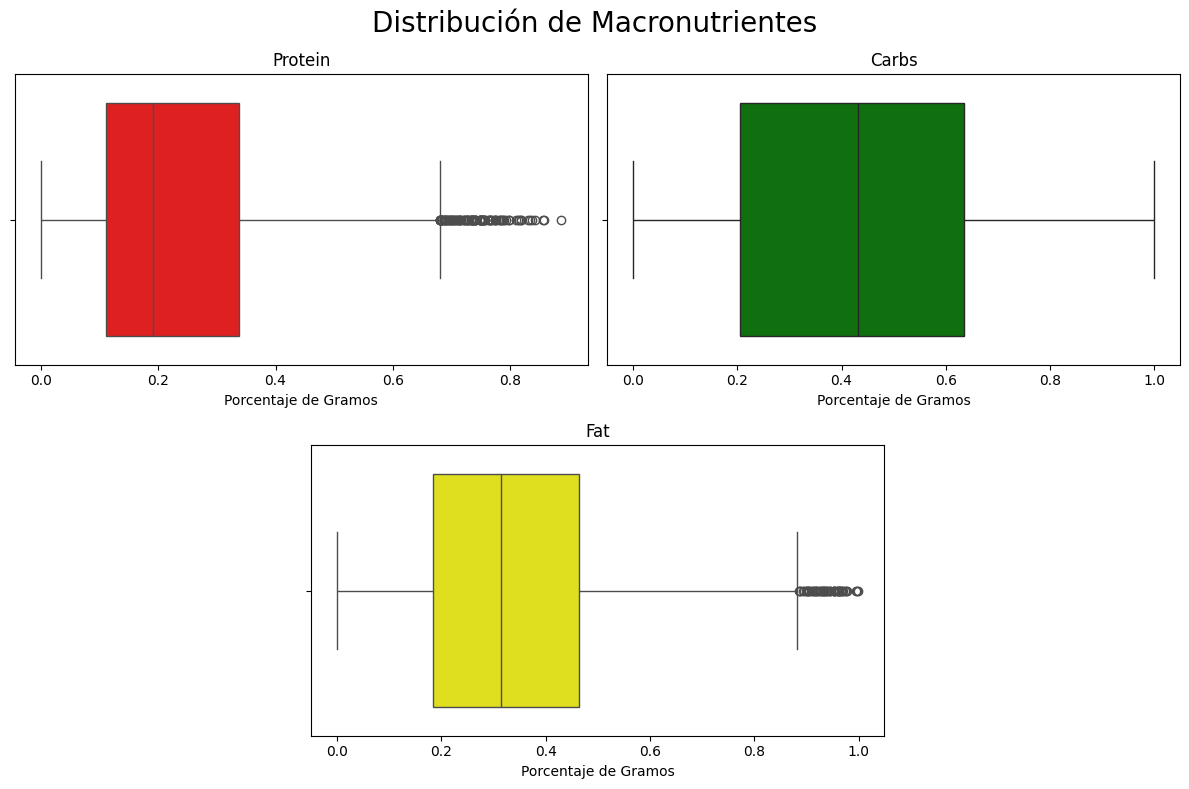
\includegraphics[width=0.75\textwidth]{Resources/2_02_plot_01.png}
    \end{center}

    Debido a que existe la presencia de datos atípicos, lo más adecuado es tratarlos 
    de manera estratificada, por tipo de dieta. Esto debido a que tratarlos de manera 
    general podría evocar que ciertas dietas queden menos representadas en comparación 
    con otras o que incluso se pierda información para consecuentes procesos. Y al 
    tratar los valores atípicos dentro de cada dieta permite reducir el impacto de 
    perder información valiosa y se siga conservando las recetas relevantes para una dieta.

    \subsection{Estratificación de Valores Cuantitativos}
    La variable Diet\_type es la principal que se emplea para 
    estratificación de las recetas, debido a que permite seprarlas 
    según una criterio bien definida, a qué dieta pertenece. Para cada 
    una de las cinco dietas se presentan los datos tabulados de sus 
    medidas de tendencia central y dispersión junto con su histograma 
    de los valores en sus macronutrientes.\\

    \subsubsection{Dieta DASH}
        \begin{center}
            \begin{tabular}{|c|ccc|}
                \hline
                Medida & Carbs(g) & Protein(g) & Fat(g) \\
                \hline
                Media               & 0.549425 & 0.196241 & 0.254334  \\
                $Q_1$               & 0.331143 & 0.068931 & 0.103381  \\
                $Q_2$               & 0.555219 & 0.156626 & 0.234742  \\
                $Q_3$               & 0.757917 & 0.282629 &	0.371292  \\
                Desviación Estándar & 0.278850 & 0.162871 & 0.194078  \\
                Mínimo              & 0.001526 & 0.000000 & 0.000000  \\
                Máximo              & 1.000000 & 0.833467 & 0.973404  \\
                Asimetría de Fisher & 0.189556 & 0.922401 & 0.461455  \\
                \hline
            \end{tabular}
            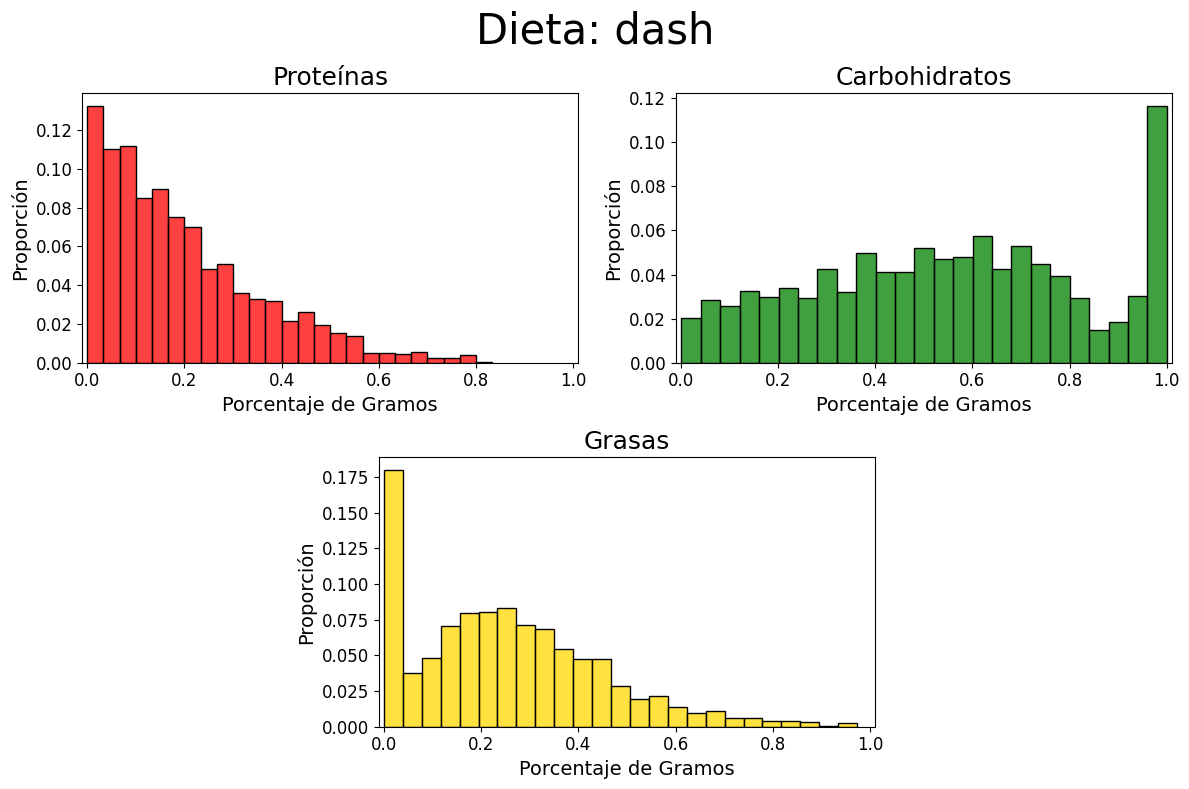
\includegraphics[width=0.75\textwidth]{Resources/2_03_plot_01.png}
        \end{center}

    \subsubsection{Dieta Keto}
        \begin{center}
            \begin{tabular}{|c|ccc|}
                \hline
                Medida & Carbs(g) & Protein(g) & Fat(g) \\
                \hline
                Media               & 0.200879 & 0.301777 & 0.497344  \\
                $Q_1$               & 0.085517 & 0.158284 & 0.405354  \\
                $Q_2$               & 0.157348 & 0.302900 & 0.505751  \\
                $Q_3$               & 0.267535 & 0.409453 & 0.591887  \\
                Desviación Estándar & 0.160609 & 0.167027 & 0.166572  \\
                Mínimo              & 0.002060 & 0.000000 & 0.000000  \\
                Máximo              & 1.000000 & 0.856868 & 0.997940  \\
                Asimetría de Fisher & 0.189556 & 0.922401 & 0.461455  \\
                \hline
            \end{tabular}
            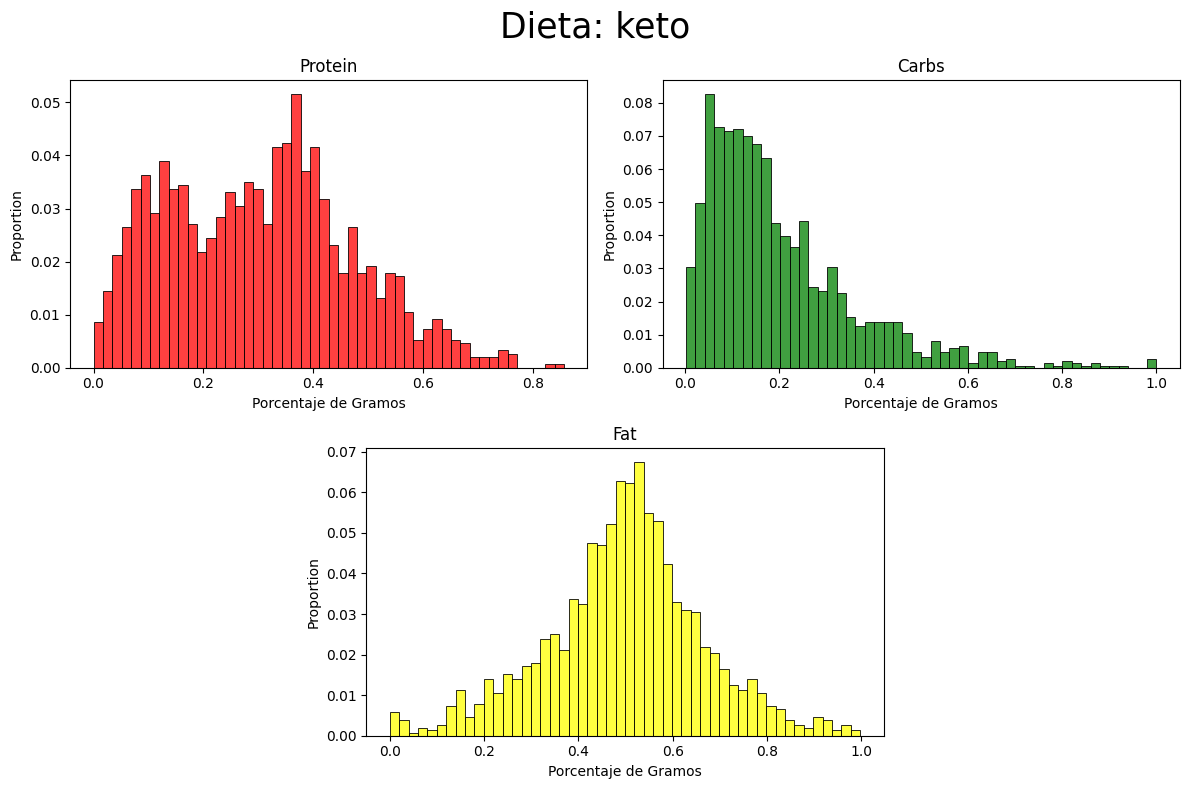
\includegraphics[width=0.75\textwidth]{Resources/2_03_plot_02.png}
        \end{center}

    \subsubsection{Dieta Mediterránea}
        \begin{center}
            \begin{tabular}{|c|ccc|}
                \hline
                Medida & Carbs(g) & Protein(g) & Fat(g) \\
                \hline
                Media               & 0.424493 & 0.279357 & 0.296150  \\
                $Q_1$               & 0.249955 & 0.159633 & 0.180357  \\
                $Q_2$               & 0.439382 & 0.227883 & 0.268336  \\
                $Q_3$               & 0.607531 & 0.377820 & 0.390404  \\
                Desviación Estándar & 0.214325 & 0.162853 & 0.160783  \\
                Mínimo              & 0.006733 & 0.005036 & 0.001731  \\
                Máximo              & 0.992746 & 0.887557 & 0.968722  \\
                Asimetría de Fisher & 0.189556 & 0.922401 & 0.461455  \\
                \hline
            \end{tabular}
            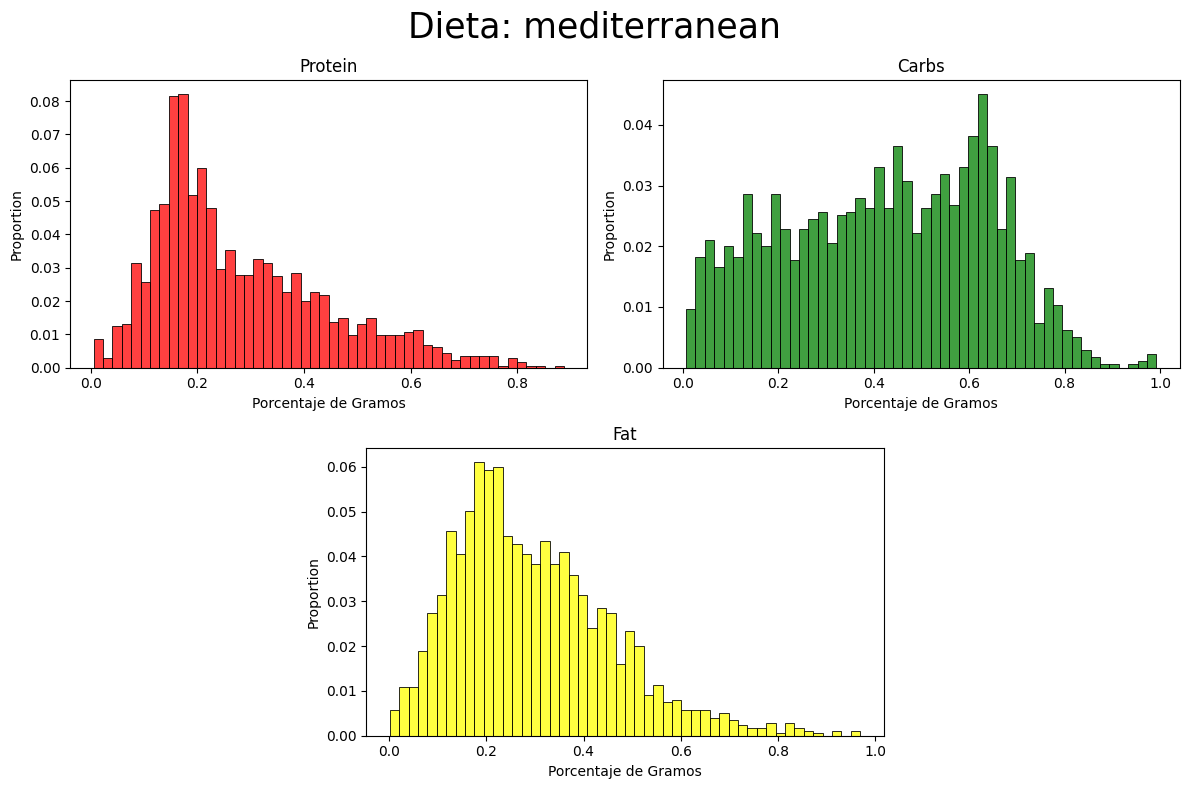
\includegraphics[width=0.75\textwidth]{Resources/2_03_plot_03.png}
        \end{center}

    \subsubsection{Dieta Paleo}
        \begin{center}
            \begin{tabular}{|c|ccc|}
                \hline
                Medida & Carbs(g) & Protein(g) & Fat(g) \\
                \hline
                Media               & 0.371307 & 0.249693 & 0.379000  \\
                $Q_1$               & 0.192399 & 0.102963 & 0.256579  \\
                $Q_2$               & 0.351300 & 0.205532 & 0.382447  \\
                $Q_3$               & 0.515054 & 0.375392 & 0.488116  \\
                Desviación Estándar & 0.221506 & 0.175031 & 0.175471  \\
                Mínimo              & 0.003612 & 0.000000 & 0.001404  \\
                Máximo              & 0.987368 & 0.858503 & 0.968835  \\
                Asimetría de Fisher & 0.189556 & 0.922401 & 0.461455  \\
                \hline
            \end{tabular}
            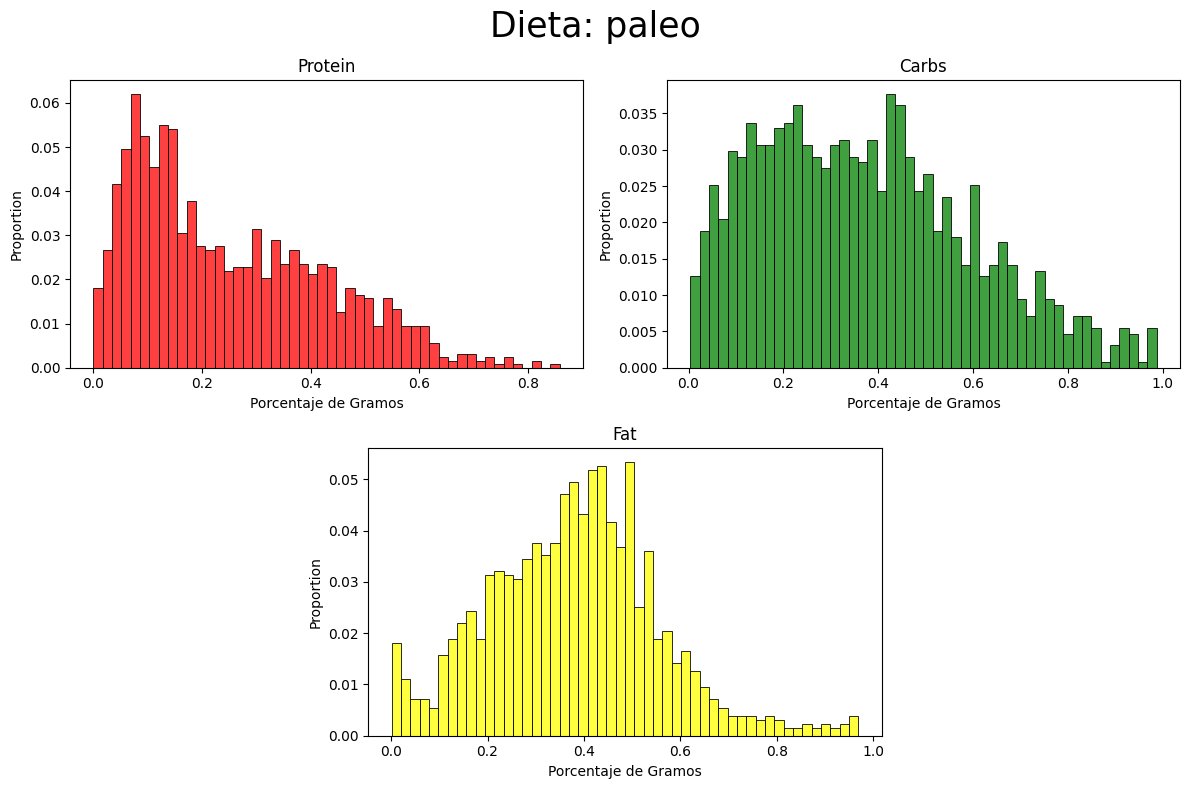
\includegraphics[width=0.75\textwidth]{Resources/2_03_plot_04.png}
        \end{center}

    \subsubsection{Dieta Vegana}
        \begin{center}
            \begin{tabular}{|c|ccc|}
                \hline
                Medida & Carbs(g) & Protein(g) & Fat(g) \\
                \hline
                Media               & 0.593968 & 0.148489 & 0.257543  \\
                $Q_1$               & 0.504070 & 0.085339 & 0.142575  \\
                $Q_2$               & 0.626246 & 0.139688 & 0.231518  \\
                $Q_3$               & 0.714679 & 0.190381 & 0.344529  \\
                Desviación Estándar & 0.171203 & 0.086088 & 0.160277  \\
                Mínimo              & 0.000330 & 0.001921 & 0.000112  \\
                Máximo              & 0.986872 & 0.647416 & 0.994887  \\
                Asimetría de Fisher & 0.189556 & 0.922401 & 0.461455  \\
                \hline
            \end{tabular}
            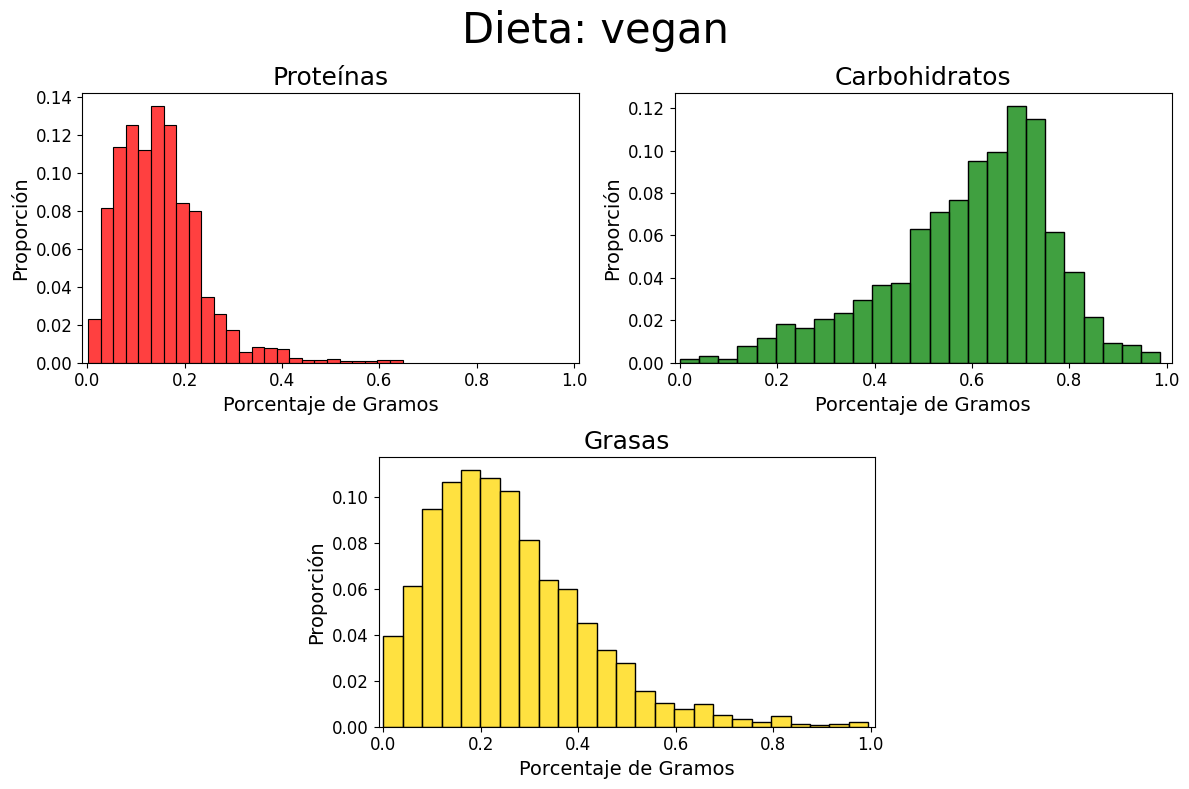
\includegraphics[width=0.75\textwidth]{Resources/2_03_plot_05.png}
        \end{center}

    \subsubsection{Gráfico de Cajas y Bigotes de la distribución de Macronutrientes por Dieta}
        \begin{center}
            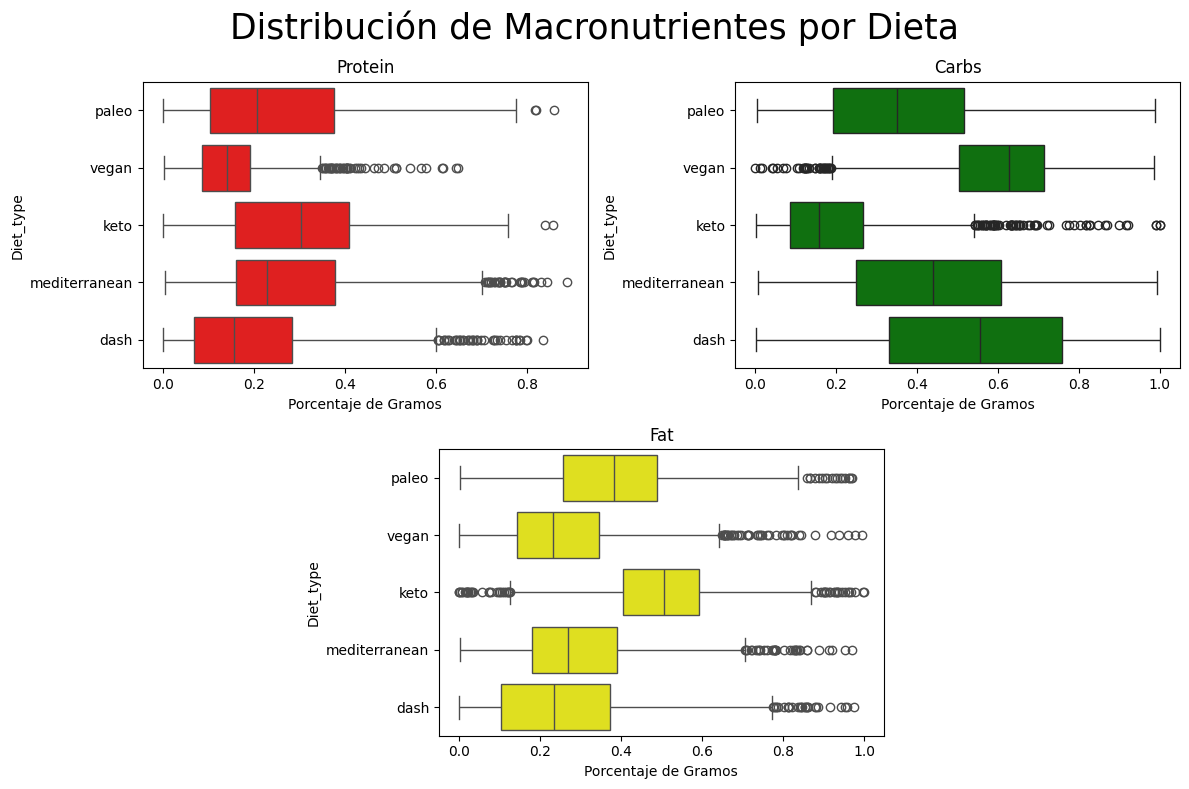
\includegraphics[width=0.75\textwidth]{Resources/2_03_plot_06.png}
        \end{center}

\newpage

\section{Muestreo e Intervalos de Confianza}

\newpage

\end{document}